\documentclass[11pt,a4paper]{article}
\usepackage[T1]{fontenc}
\usepackage[margin=2.3cm]{geometry}
\usepackage{amsmath,amssymb}
\usepackage{graphicx}
\usepackage[dvipsnames]{xcolor}
\usepackage{enumitem}
\usepackage[colorlinks=true,linkcolor=blue,urlcolor=blue]{hyperref}
\setlength{\parskip}{0.6em}
\setlength{\parindent}{0pt}
\begin{document}

\begin{center}{\LARGE\bfseries opengyro}\\[0.4em]{\large Why a spinning top does not fall: torque, angular momentum and precession, in three sessions.}\\[0.2em]\small PAN IIT OSS explainer \textbullet{} secondary school to diploma / undergraduate (levels 3-5)\end{center}

\section*{Why this exists}
A spinning top does not fall because gravity changes the direction of its angular momentum instead of its length. This explainer builds that idea from arrows to a formula to a simulation, using only basic mechanics and a little calculus.

\section*{The end goal}
Explain a spinning top's precession. The end goal is to explain a spinning top's precession: why it circles, how fast, and when it stops being stable. The same mathematics governs gyroscopes in navigation, spinning satellites and the precession of the Earth's axis.

\section*{How the three sessions build up}
\begin{enumerate}[nosep]
\item \textbf{Session 1: A spinning wheel resists being tilted} (Level 1, conceptual interactive model, 60 min).
\item \textbf{Session 2: The precession formula and a design problem} (Level 2, mathematical engineering model, 75 min).
\item \textbf{Session 3: Simulating the heavy top: Euler angles, precession and nutation} (Level 3, simulation and validation, 90 min).
\end{enumerate}

\section{Session 1: A spinning wheel resists being tilted}

\subsection*{A. Real-world problem}
Hold a bicycle wheel by one end of its axle, with the axle horizontal. If the wheel is not spinning, the axle flops down at once. Get the wheel spinning fast and the axle stays up, and then does something odd: it swings slowly round in a horizontal circle. A spinning top does the same thing: it does not fall over while it spins, it slowly circles. Why does the wheel go sideways when gravity pulls it down? This is general education about everyday rotating objects; the models here are simplified.

\subsection*{B. Concept and theory}
A spinning wheel has angular momentum L, an arrow along its axle (right-hand rule: curl the fingers along the spin and the thumb gives the direction). Its size is L = I w, where w is the spin in radians per second and I is the moment of inertia: how hard the wheel is to spin up. A push that tries to turn the wheel is a torque, also an arrow. The rule that governs everything is: the change of L in a short time is the torque times that time. Gravity pulls the wheel's centre down, a distance r from the support. That gives a torque of size m g r that points sideways, at right angles to the axle (not down!). A change of L at right angles to L cannot make the arrow longer; it only turns it. So the axle swings round in a horizontal circle. The turning rate is torque divided by L, so a faster spin (bigger L) means a slower circling.

\begin{itemize}[nosep]
\item w: spin of the wheel about its axle (rad/s)
\item I: moment of inertia about the axle (disc: m R\textasciicircum{}2 / 2) (kg m\textasciicircum{}2)
\item L: angular momentum, L = I w (kg m\textasciicircum{}2/s)
\item tau: torque of the weight about the support, m g r (N m)
\item r: distance from the support to the wheel centre (m)
\item Omega\_p: circling rate of the axle (precession) (rad/s)
\end{itemize}

\begin{equation*}
L = I\,w
\end{equation*}

\begin{equation*}
\tau = m g r
\end{equation*}

\begin{equation*}
\Delta \mathbf L = \boldsymbol\tau\,\Delta t
\end{equation*}

\begin{equation*}
\Omega_p = \frac{\tau}{L}
\end{equation*}

\begin{center}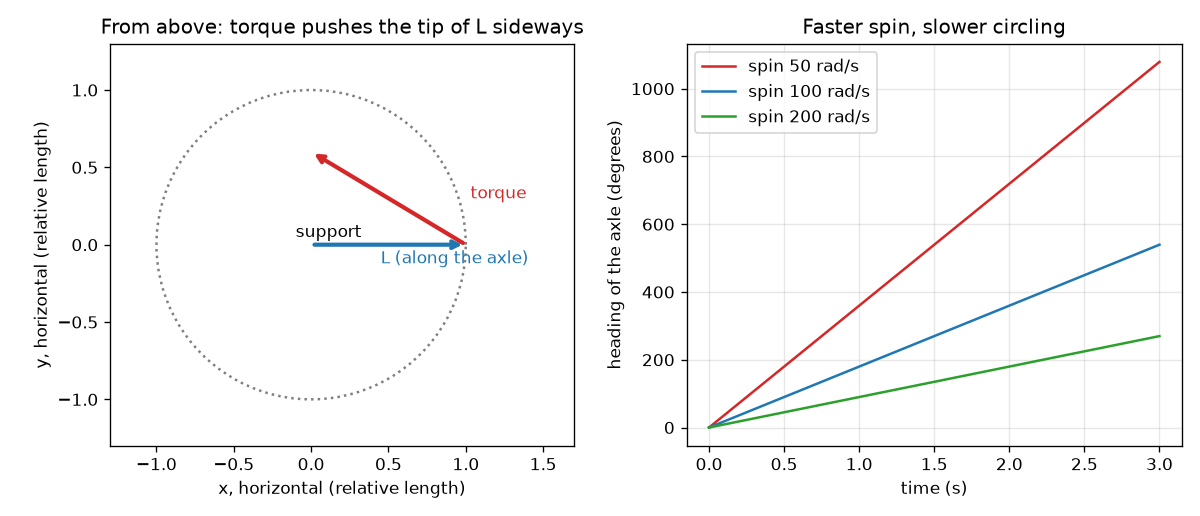
\includegraphics[width=0.85\linewidth]{figures/s01_torque_and_L.png}\\\small Left: from above, the torque (red) pushes the tip of L (blue) sideways. Right: heading against time for three spin rates; a faster spin circles more slowly.\end{center}

\subsection*{E. Worked example}
For the wheel above (0.5 kg, radius 5 cm, centre 4 cm from the support) spinning at 100 rad/s, find L, the torque, the circling rate and the time for one circle.
\begin{enumerate}[nosep]
\item I = m R\textasciicircum{}2 / 2 = 0.5 * 0.05\textasciicircum{}2 / 2 = 6.25e-4 kg m\textasciicircum{}2.
\item L = I w = 6.25e-4 * 100 = 0.0625 kg m\textasciicircum{}2/s.
\item tau = m g r = 0.5 * 9.81 * 0.04 = 0.1962 N m.
\item Omega\_p = tau / L = 0.1962 / 0.0625 = 3.139 rad/s.
\item One circle is 2 pi radians, so it takes 2 pi / 3.139 = 2.00 s.
\end{enumerate}
\textbf{Answer.} L = 0.0625 kg m\textasciicircum{}2/s, torque 0.1962 N m, circling 3.139 rad/s, one circle in 2.00 s. At 200 rad/s the same wheel circles at 1.570 rad/s (4.00 s).

\subsection*{F. Questions}
\begin{enumerate}[nosep]
\item \textbf{Conceptual.} Gravity pulls the wheel down. Why does the axle move sideways instead of down?
\item \textbf{Numerical.} A wheel has I = 0.02 kg m\textasciicircum{}2 and spins at 50 rad/s. Find L. What is the circling rate if the torque of its weight is 0.30 N m?
\item \textbf{Graph and simulation interpretation.} In the heading graph, the line for 200 rad/s is half as steep as the line for 100 rad/s. What does that tell you about the relation between spin and circling rate?
\item \textbf{Design and optimisation challenge.} Design: you want the axle of this wheel to circle once every 2 seconds. Which spin do you need? Would it work for a person's hand-held spin of about 60 rad/s?
\end{enumerate}

\section{Session 2: The precession formula and a design problem}

\subsection*{A. Real-world problem}
A demonstrator holds a solid-disc wheel (mass 2 kg, radius 0.30 m) by an axle whose support is 0.25 m from the wheel centre. The wheel is spun and the axle swings slowly round. Can we choose the spin rate so that the axle makes exactly one circle every 4 seconds, and is that a spin a person can reach by hand? General education only: this is a simplified classroom model, not a design method for real machinery.

\subsection*{B. Concept and theory}
Newton's second law for rotation: the torque equals the rate of change of the angular momentum vector, tau = dL/dt. For a horizontal axle held at one end, the weight m g acts at the centre, r from the support, so tau = m g r, horizontal and at right angles to L. Then L keeps its size L = I w and only turns: in time dt it turns through the angle dphi = tau dt / L. So Omega\_p = dphi/dt = tau / L = m g r / (I w). A solid disc has I = m R\textasciicircum{}2 / 2, so Omega\_p = 2 g r / (R\textasciicircum{}2 w): the mass drops out. The formula needs a fast spin: the exact steady precession of a symmetric top at angle theta from the upward vertical solves I1 cos(theta) Omega\textasciicircum{}2 - I3 w Omega + m g r = 0 (derived in Session 3), where I1 = m R\textasciicircum{}2 / 4 + m r\textasciicircum{}2 for a disc about the support. It exists only when (I3 w)\textasciicircum{}2 \textgreater{}= 4 I1 m g r cos(theta); the fast-spin formula is the slow root when I3 w is much bigger than the square root of 4 I1 m g r. At a horizontal axle (theta = 90 degrees) the formula is exact. The fast-spin ratio (I3 w)\textasciicircum{}2 / (4 I1 m g r) tells how safely the formula applies.

\begin{itemize}[nosep]
\item m: mass of the wheel (kg)
\item R: radius of the wheel (m)
\item r: distance from the support to the wheel centre (m)
\item g: gravitational acceleration, 9.81 (m/s\textasciicircum{}2)
\item w: spin about the axle (rad/s)
\item I: moment of inertia about the axle (kg m\textasciicircum{}2)
\item Omega\_p: precession rate (rad/s)
\item T: time for one circle, 2 pi / Omega\_p (s)
\end{itemize}

\begin{equation*}
I_{\mathrm{disc}} = \tfrac12 m R^2
\end{equation*}

\begin{equation*}
\boldsymbol\tau = \frac{d\mathbf L}{dt},\qquad \tau = m g r,\qquad L = I w
\end{equation*}

\begin{equation*}
\Omega_p = \frac{m g r}{I w} = \frac{2 g r}{R^2 w}\quad\text{(solid disc)}
\end{equation*}

\begin{equation*}
w = \frac{m g r\,T}{2\pi I}\quad\text{(spin for one circle in time } T\text{)}
\end{equation*}

\begin{equation*}
I_1\cos\theta\,\Omega^2 - I_3 w\,\Omega + m g r = 0
\end{equation*}

\begin{center}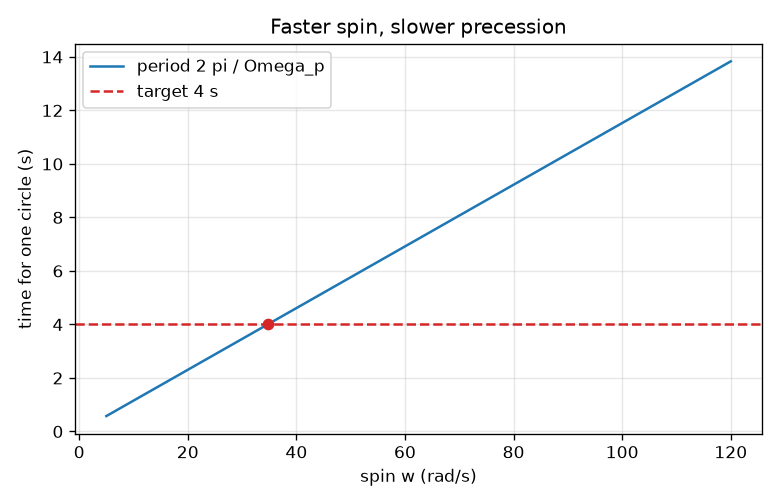
\includegraphics[width=0.85\linewidth]{figures/s02_period_vs_spin.png}\\\small Time for one circle against spin: a straight line; the target of 4 s needs 34.7 rad/s.\end{center}

\subsection*{E. Worked example}
Wheel: m = 2.0 kg, R = 0.30 m, r = 0.25 m, solid disc. Find the spin for one circle every 4 s, in rad/s and rpm, and check the result.
\begin{enumerate}[nosep]
\item I = m R\textasciicircum{}2 / 2 = 2.0 * 0.09 / 2 = 0.0900 kg m\textasciicircum{}2.
\item Target rate: Omega\_p = 2 pi / 4 = 1.5708 rad/s.
\item Torque: tau = m g r = 2.0 * 9.81 * 0.25 = 4.905 N m.
\item L = tau / Omega\_p = 4.905 / 1.5708 = 3.123 kg m\textasciicircum{}2/s, so w = L / I = 3.123 / 0.0900 = 34.70 rad/s.
\item In rpm: 34.70 * 60 / (2 pi) = 331 rpm, about 5.5 turns per second.
\item Check: Omega\_p = m g r / (I w) = 4.905 / (0.09 * 34.70) = 1.5708 rad/s, period 4.000 s. Half the spin gives 2.00 s, double gives 8.00 s.
\end{enumerate}
\textbf{Answer.} w = 34.70 rad/s = 331 rpm (L = 3.123 kg m\textasciicircum{}2/s). The formula is exact for a horizontal axle; for an axle tilted 60 degrees from the vertical the exact rate at this spin is 1.644 rad/s instead of 1.571 (4.7 percent more).

\subsection*{F. Questions}
\begin{enumerate}[nosep]
\item \textbf{Conceptual.} Why does a faster spin give a slower precession? And why does the mass not matter for a solid disc of fixed radius?
\item \textbf{Numerical.} A solid-disc wheel with m = 1.0 kg, R = 0.20 m, r = 0.30 m spins at 50 rad/s about a horizontal axle. Find I, Omega\_p and the time for one circle.
\item \textbf{Graph and simulation interpretation.} In the period-versus-spin graph (m = 2 kg, R = 0.30 m, r = 0.25 m) the line passes through (34.7, 4). What is its slope, and what would the period be at 17 rad/s?
\item \textbf{Design and optimisation challenge.} Design: a real bicycle wheel has its mass on the rim, so I is about m R\textasciicircum{}2, twice the disc value. With the same m, R and r, what spin gives a 4 s circle? What stays the same? Which is easier to produce by hand, and what is the trade-off?
\end{enumerate}

\section{Session 3: Simulating the heavy top: Euler angles, precession and nutation}

\subsection*{A. Real-world problem}
A toy top spun fast at a tilt does not fall: it circles slowly (precession) and shivers a little (nutation). Spun slowly it topples. Spun upright and fast enough it stands still, 'sleeping'. Can a simulation reproduce all three, and can we trust it? We do not experiment on a real top here: this is a frictionless textbook model, simplified, and real tops slow down and wobble because of friction.

\subsection*{B. Concept and theory}
A rigid body turns about a fixed point O (the tip). Three Euler angles describe it: theta is the tilt of the symmetry axis from the upward vertical, phi turns the axis around the vertical, and psi is the spin about the axis. The body is symmetric: I3 about the axis, I1 about any perpendicular axis through O. With w3 = psi' + phi' cos(theta) (the spin component along the axis) the kinetic energy is I1/2 (theta'\textasciicircum{}2 + phi'\textasciicircum{}2 sin\textasciicircum{}2 theta) + I3/2 w3\textasciicircum{}2 and the potential energy is m g r cos(theta), so the Lagrangian is L = T - V. The angles phi and psi do not appear in L, hence p\_psi = I3 w3 and p\_phi = I1 phi' sin\textasciicircum{}2 theta + I3 w3 cos(theta) are constant (Noether). The Lagrange equation for theta gives theta'' = phi'\textasciicircum{}2 sin(theta) cos(theta) - (I3/I1) w3 phi' sin(theta) + (m g r / I1) sin(theta), and differentiating p\_phi gives phi''; psi'' follows from w3 constant. We integrate all with RK4 and then check that energy, p\_phi and p\_psi stay constant. For a fast spin the theory gives a slow precession Omega\_p = m g r / (I3 w3) and a fast nutation at about w\_n = I3 w3 / I1. A top that is nearly vertical is stable (sleeps) if w3\textasciicircum{}2 \textgreater{} 4 m g r I1 / I3\textasciicircum{}2: this is the standard classical stability bound for a vertical top, which we verify numerically rather than derive.

\begin{itemize}[nosep]
\item theta, phi, psi: Euler angles: tilt, turn about the vertical, spin about the axis (rad)
\item w3: spin component along the axis, psi' + phi' cos(theta) (rad/s)
\item I3, I1: moments of inertia about the symmetry axis and a perpendicular axis through the tip (kg m\textasciicircum{}2)
\item m g r: largest gravity torque (r: tip to centre of mass) (N m)
\item p\_phi, p\_psi: conserved angular momentum components (kg m\textasciicircum{}2/s)
\item Omega\_p, w\_n: precession rate and nutation frequency (rad/s)
\end{itemize}

\begin{equation*}
\mathcal L = \tfrac12 I_1\left(\dot\theta^2 + \dot\phi^2\sin^2\theta\right) + \tfrac12 I_3\left(\dot\psi + \dot\phi\cos\theta\right)^2 - m g r\cos\theta
\end{equation*}

\begin{equation*}
p_\psi = I_3 \omega_3,\qquad p_\phi = I_1\dot\phi\sin^2\theta + I_3\omega_3\cos\theta,\qquad \omega_3=\dot\psi+\dot\phi\cos\theta
\end{equation*}

\begin{equation*}
\ddot\theta = \dot\phi^2\sin\theta\cos\theta - \frac{I_3}{I_1}\omega_3\dot\phi\sin\theta + \frac{m g r}{I_1}\sin\theta
\end{equation*}

\begin{equation*}
E = \tfrac12 I_1\left(\dot\theta^2 + \dot\phi^2\sin^2\theta\right) + \tfrac12 I_3\omega_3^2 + m g r\cos\theta
\end{equation*}

\begin{equation*}
\Omega_p \approx \frac{m g r}{I_3\omega_3},\qquad \omega_n \approx \frac{I_3\omega_3}{I_1}
\end{equation*}

\begin{equation*}
\omega_3^2 > \frac{4 m g r\, I_1}{I_3^2}\quad\text{(sleeping top, classical result)}
\end{equation*}

\begin{center}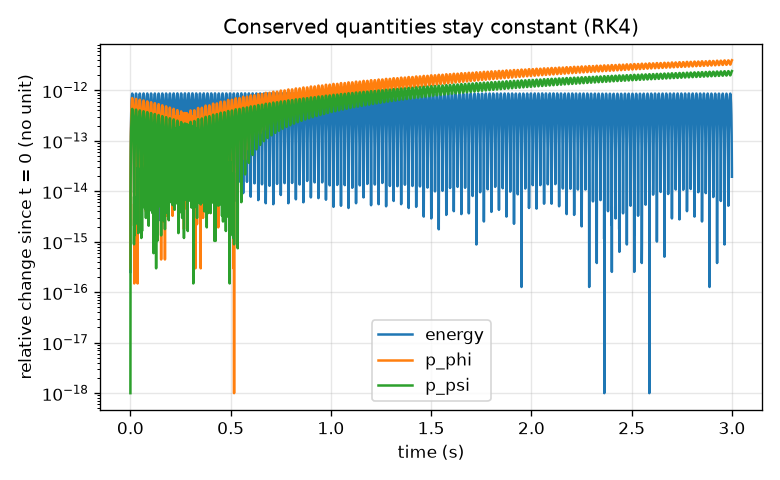
\includegraphics[width=0.85\linewidth]{figures/s03_conservation.png}\\\small Relative change of energy, p\_phi and p\_psi stays tiny over 3 s (RK4, 0.2 ms steps).\end{center}

\subsection*{E. Worked example}
Top: m = 0.5 kg, R = 5 cm, r = 4 cm, spin w3 = 300 rad/s, released at 60 degrees. Predict the precession rate, its period and the nutation frequency, then compare with the simulation.
\begin{enumerate}[nosep]
\item I3 = m R\textasciicircum{}2 / 2 = 6.25e-4 kg m\textasciicircum{}2; I1 = m R\textasciicircum{}2 / 4 + m r\textasciicircum{}2 = 3.125e-4 + 8.0e-4 = 1.1125e-3 kg m\textasciicircum{}2; m g r = 0.5 * 9.81 * 0.04 = 0.1962 N m.
\item I3 w3 = 6.25e-4 * 300 = 0.1875 kg m\textasciicircum{}2/s.
\item Precession: Omega\_p = 0.1962 / 0.1875 = 1.0464 rad/s, so one circle takes 2 pi / 1.0464 = 6.00 s.
\item Nutation: w\_n = I3 w3 / I1 = 0.1875 / 1.1125e-3 = 168.5 rad/s, i.e. 26.8 per second.
\item Simulation (RK4, dt = 0.2 ms, 3 s): precession 1.0496 rad/s (0.3 percent above the formula), nutation 167.5 rad/s (0.6 percent below).
\item Validation: relative drift of p\_psi, p\_phi and energy is below 1e-11.
\end{enumerate}
\textbf{Answer.} Formula: 1.046 rad/s (period 6.00 s) and nutation 168.5 rad/s; simulation: 1.050 rad/s and 167.5 rad/s. They agree within about 1 percent. At 80 rad/s the formula is 3.2 percent low, at 600 rad/s only 0.1 percent.

\subsection*{F. Questions}
\begin{enumerate}[nosep]
\item \textbf{Conceptual.} The simulation does not build conservation into the integration. Why is it still a good test that p\_phi, p\_psi and the energy stay constant?
\item \textbf{Numerical.} Use the classical bound w3\textasciicircum{}2 \textgreater{} 4 m g r I1 / I3\textasciicircum{}2 to find the minimum spin for a vertical top for this disc (m = 0.5 kg, r = 4 cm, I1 = 1.1125e-3, I3 = 6.25e-4 kg m\textasciicircum{}2).
\item \textbf{Graph and simulation interpretation.} In the tilt-versus-time graph at 300 rad/s the tilt ripples with a period of about 0.037 s while the axis circles once in about 6 s. What do these two periods tell you about Omega\_p and w\_n?
\item \textbf{Design and optimisation challenge.} Design: a toy maker pulls a string that gives at most 120 rad/s. The top (same disc) must stand safely above the sleeping limit (use a 30 percent margin) and precess slower than 3 rad/s when tilted. Choose a spin and justify it.
\end{enumerate}

\section{Real-world mini-project}
\textbf{Tune a gyroscope to precess at a target rate.} A demonstration gyroscope (the 0.5 kg, 5 cm disc of Session 3, centre 4 cm from the support, released from a 60 degree tilt with zero precession speed) must circle at 2.0 rad/s, one circle every 3.14 s. Start from the formula m g r / (I w) to get a first spin rate, then use \texttt{simulate} and \texttt{measured\_rates} from Session 3 to refine the spin until the simulated mean precession rate is within 0.5 percent of 2.0 rad/s.

\section{The path ahead}
\begin{enumerate}[nosep]
\item \textbf{Session 4: A top that can start exactly vertical.} The same top integrated with a quaternion for the attitude and the body-frame Euler equations.
\item \textbf{Session 5: Predict the mean precession from the effective potential.} A function that predicts the nutation range and the mean precession rate without running the time loop.
\item \textbf{Session 6: Spin-down and the start of the wobble.} A simulation in which the spin decays exponentially (time constant 8 s) from 100 rad/s.
\item \textbf{Session 7: A 3D view with the tip trace.} An animated top with the trace of the axis tip, the L arrow and a live precession plot.
\item \textbf{Session 8: Torque-free tumbling: the tennis racket effect.} A body with three different moments of inertia simulated with the Euler equations.
\end{enumerate}

\section{Answers and hints}

\subsection*{Session 1}
\begin{enumerate}[nosep]
\item \textbf{Conceptual.} Hint: Which way does the torque of gravity point, and what does a change of L at right angles to L do to the arrow? Solution: The torque of the weight about the support is horizontal and at right angles to the axle. The rule says the change of L is the torque times the time, so L changes sideways. A sideways change of an arrow rotates it without changing its length, so the axle swings round horizontally. Without spin there is no L to steer, so gravity just tips the wheel down.
\item \textbf{Numerical.} Hint: L = I w, then Omega\_p = torque / L. Check the units. Solution: L = 0.02 * 50 = 1.0 kg m\textasciicircum{}2/s. Omega\_p = 0.30 / 1.0 = 0.30 rad/s, i.e. one circle in 2 pi / 0.30 = 20.9 s. Units: N m divided by kg m\textasciicircum{}2/s is 1/s, i.e. rad/s. Sanity check: a heavy wheel spun this fast circles slowly.
\item \textbf{Graph and simulation interpretation.} Hint: Slope of the heading line is the circling rate. Solution: The slope is the circling rate and it is inversely proportional to the spin: doubling the spin halves the rate (3.139 to 1.570 rad/s). This follows from Omega\_p = torque / (I w). A straight line means the rate is constant.
\item \textbf{Design and optimisation challenge.} Hint: Required rate is 2 pi / 2 rad/s; then w = torque / (I Omega\_p). Solution: Omega\_p = 2 pi / 2 = 3.1416 rad/s, w = 0.1962 / (6.25e-4 * 3.1416) = 99.9 rad/s, about 100 rad/s (955 rpm). A hand spin of 60 rad/s gives one circle every 1.2 s, too fast. Trade-off: a faster spin needs a motor or a string pull; a heavier wheel (bigger I) reaches the same L at a lower spin.
\end{enumerate}

\subsection*{Session 2}
\begin{enumerate}[nosep]
\item \textbf{Conceptual.} Hint: Omega\_p = tau / L. What happens to each of tau and L when the spin or the mass changes? Solution: The torque of gravity is fixed by m g r, while L = I w grows with the spin, so the arrow L turns by a smaller angle each second. For a disc both the torque and I are proportional to m, so m cancels: Omega\_p = 2 g r / (R\textasciicircum{}2 w). A heavier disc has a bigger torque but also resists being turned by exactly as much.
\item \textbf{Numerical.} Hint: I = m R\textasciicircum{}2 / 2. Then Omega\_p = m g r / (I w) and T = 2 pi / Omega\_p. Solution: I = 1.0 * 0.04 / 2 = 0.020 kg m\textasciicircum{}2. Omega\_p = 1.0 * 9.81 * 0.30 / (0.020 * 50) = 2.943 rad/s. T = 2 pi / 2.943 = 2.135 s. Units: N m divided by kg m\textasciicircum{}2/s is 1/s. Sanity check: 50 rad/s is only 8 turns per second, so a quick circle is plausible.
\item \textbf{Graph and simulation interpretation.} Hint: The line is T = 2 pi I w / (m g r), so the slope is T / w. Solution: Slope = 4 / 34.7 = 0.1153 s per (rad/s) (the formula gives 2 pi * 0.09 / 4.905 = 0.1153). At 17 rad/s T = 0.1153 * 17 = 1.96 s. The straight line through the origin says period is proportional to spin. But near and below about 20 rad/s this wheel has no steady precession when tilted, and the fast-spin ratio is close to 1, so the formula should not be trusted there.
\item \textbf{Design and optimisation challenge.} Hint: w = m g r T / (2 pi I). What does L = tau / Omega\_p depend on? Solution: With I = 0.18 kg m\textasciicircum{}2: w = 4.905 * 4 / (2 pi * 0.18) = 17.35 rad/s = 166 rpm, half the disc value. L = tau / Omega\_p = 3.123 kg m\textasciicircum{}2/s is the same: the target rate fixes L, and a larger I only lowers the spin needed. A hand can reach 166 rpm more easily than 331 rpm. Trade-off: the rim-heavy wheel is harder to spin up and to hold, and the fast-spin condition should be re-checked with the right I1.
\end{enumerate}

\subsection*{Session 3}
\begin{enumerate}[nosep]
\item \textbf{Conceptual.} Hint: The RK4 steps are only an approximation of the equations; what does it mean if a conserved quantity drifts? Solution: The equations of motion were derived from L, so exact solutions conserve all three. The integrator knows nothing about them, so any drift measures its error, and a mistake in the equations (a wrong sign or factor) would make them drift at once. A small drift (below 1e-11 here) does not prove the formulas are right, but a large drift proves something is wrong.
\item \textbf{Numerical.} Hint: w3\_min = sqrt(4 m g r I1) / I3. Solution: 4 * 0.1962 * 1.1125e-3 = 8.731e-4; its square root is 0.02955; divided by 6.25e-4 this is 47.3 rad/s (452 rpm). The simulation agrees: released 2.9 degrees off vertical, 1.3 times the limit (61.5 rad/s) never tilts more than 4.5 degrees, while 0.8 times the limit (37.8 rad/s) tips over to 73.9 degrees.
\item \textbf{Graph and simulation interpretation.} Hint: Frequency is 2 pi divided by the period. Solution: The ripple (nutation) has w\_n = 2 pi / 0.037 = 170 rad/s, matching I3 w3 / I1 = 168.5 rad/s, and the slow circle has Omega\_p = 2 pi / 6 = 1.05 rad/s. Nutation is about 160 times faster than precession, which is why for a fast spin the top seems to move smoothly: the quick shivers are tiny and average out.
\item \textbf{Design and optimisation challenge.} Hint: Two constraints: w3 \textgreater{}= 1.3 * 47.3 and Omega\_p = m g r / (I3 w3) \textless{}= 3. Solution: Margin: w3 \textgreater{}= 1.3 * 47.3 = 61.5 rad/s. Precession: w3 \textgreater{}= 0.1962 / (6.25e-4 * 3) = 104.6 rad/s. Both hold for w3 between about 105 and 120 rad/s. Choose 110 rad/s: Omega\_p = 0.1962 / (6.25e-4 * 110) = 2.85 rad/s (one circle every 2.2 s). Trade-off: a margin near 120 rad/s leaves little room for string variation; friction will lower the spin during use, so the real design also needs a slower spin-down.
\end{enumerate}

\section{How to join}
Read \texttt{CONTRIBUTING.md} in the repository, then pick an issue labelled \texttt{good first issue}. Repository: \url{https://github.com/KrunalPanchal1995/opengyro}

\end{document}
